\subsection{EXAMPLE EXPERIMENTS ON GLM}

\begin{figure}[th!]
\centering
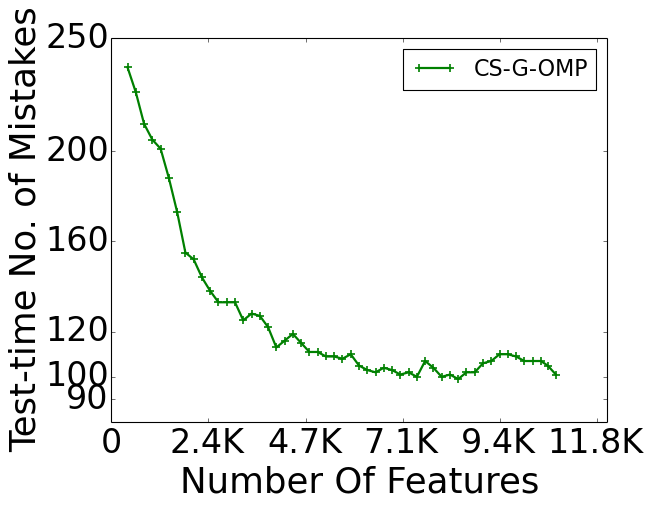
\includegraphics[width=0.8\textwidth]{\GOMPDIR/img/extra_exp_v2.png}
\caption{CS-G-OMP test-time performance on MNIST. We note that CS-G-FR cannot be computed easily in this case and is omitted.} 
\label{fig:mnist}
\end{figure}
We present here experimental results of CS-G-OMP with generalized linear models on a MNIST database of handwritten digit classification~\citep{MNIST}.
We generate features from raw digit pixels following the recent development of \cite{gem}. It  generates about 11,000 dimensional features via generalized eigenvectors of pairs of second moments of the raw pixel values of different classes, and achieves one-percent error rate with logistic regressions. We partition the generated features into 54 equal-sized random feature groups, and apply CS-G-OMP with multi-class-logistic regression, targeting the one-hot encodings of sample labels. Mathematically, we choose our mean function of generalized linear model, $\nabla \phi: \mathbb{R}^P \rightarrow \mathbb{R}^P$, as 
$\nabla \phi(x) = \frac{exp(x)}{\sum _p^P exp(x)_p}$ for Algorithm~\ref{algo:gomp_glm}, where $exp(x)$ is an element-wise exponential function. 

As shown in Figure~\ref{fig:mnist}, the test-time accuracy improves greatly at start, quickly reducing the number of mistakes below 150 (i.e., 98.5\% accuracy with the 10K test samples of MNIST) with 2200 out of the 11k total features, and plateaus between 105 and 100 mistakes with 6k features and beyond. The peak performance is 99 mistakes, and the final result has 101 mistakes.  Since logistic regression with 11K features and 60K training samples takes non-trivial time to train, the runtime gap between CS-G-OMP and CS-G-FR further widens: CS-G-OMP is able to finish the sequencing in 12 hours, while CS-G-FR takes days to progress. This is because the model training time is orders of magnitudes longer than that of computing gradient w.r.t. the coefficient matrix. In fact, one selection of CS-G-FR takes longer than the full run of CS-G-OMP. As a result, we do not report CS-G-FR result on this data-set.




